\lstset{language=json}
\chapter{Kommunikation mit Shulker-Core}
\textit{Shulker-Connect} muss mit \textit{Shulker-Core} kommunizieren, sodass eine API-Anfrage an Shulker-Connect tatsächlich
auch das Türschloss steuern kann.
Eine lokale Kommunikation zwischen mehreren Software-Lösungen kann mittels
\textit{inter process communication} umgesetzt werden. 
Um eine stabile und effiziente Kommunikation mit der auf dem Raspberry PI laufenden Rust-Software Shulker-Core zu 
gewährleisten, haben wir auf beiden Endpunkten \textit{POSIX-Sockets} implementiert.

Beim Start von Shulker-Connect werden zwei neue Threads erstellt: Ein Listener-Thread und ein Sender-Thread.
Beide Threads erstellen ein \textit{socket}-Objekt, das auf eine Verbindung von \textit{Shulker-Core} wartet.
Wird diese hergestellt, sind die Threads bereit, Daten zu senden bzw. zu empfangen.
In Shulker werden alle Nachrichten im \textit{UTF8}-Format gesendet.

\section{Was sind POSIX-Sockets?}
\textit{POSIX local inter-process communication sockets} (auch Unix Domain Sockets oder IPC Sockets genannt) ermöglichen
eine bidirektionale Kommunikationsverbindung für die Interprozesskommunikation (IPC) auf UNIX basierenden Systemen.
Hierbei wird von beiden Kommunikations-Partnern eine Datei vereinbart, über diese die Kommunikation erfolgt. \cite{ipcsockets}
Die Kommunikation zwischen Shulker-Connect und Shulker-Core muss nicht verschlüsselt werden, da eine Kompromittierung des
Raspberry-Pi's die einzige Möglichkeit darstellt, diese Kommunikation mitzulesen. 

\section{Aufbau der POSIX-Nachrichten}
Da Shulker-Connect und Shulker-Core über String-Nachrichten miteinander kommunizieren, haben wir ein
Format festgelegt, an welchen sich alle Nachrichten der Kommunikation halten müssen.


Alle gesendeten Nachrichten werden im JSON-Format gesendet. Jede JSON-Nachricht beinhaltet immer ein Attribut namens
\textit{"method"}, dieses ist der Identifikator der Anfrage und lässt sich mit Routen von Web-Diensten vergleichen.
Zusätzlich können beliebige andere Attribute, die für die jeweilige Route relevant sind, in der Nachricht mitgesendet werden.
Zu guter Letzt wird ein Nachrichtentrenner an das Ende einer jeder Nachricht gesetzt. Wir haben uns für
\textbf{"\textbackslash n"} entschieden.

\section{Ablauf einer Anfrage zu Shulker-Connect}
Um zu demonstrieren, wie der Ablauf einer Anfrage an Shulker-Connect intern gehandhabt wird, schauen wir uns das Generieren
eines Session-Tokens an.

\begin{figure}[H]
    \begin{center}
        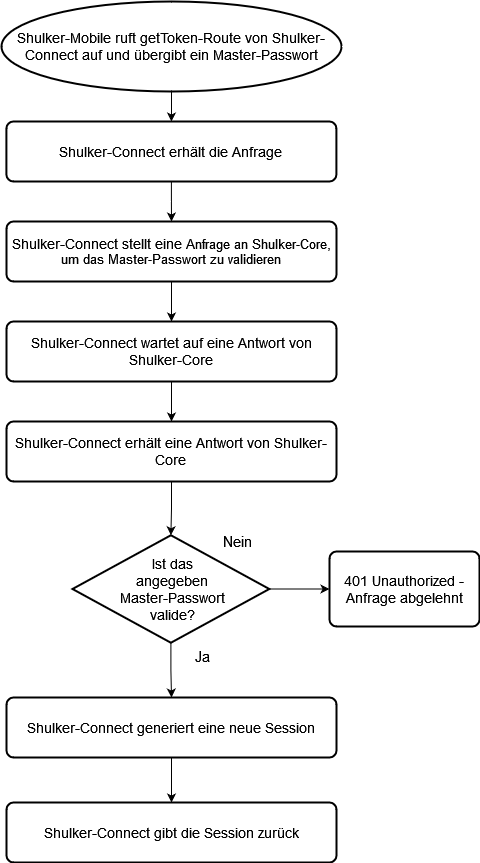
\includegraphics[width=.6\textwidth]{images/connect/AblaufGetToken.png}
        \caption{Workflow der Abfrage zum generieren einer neuen Session}
    \end{center}
\end{figure}

Als erstes ruft Shulker-Mobile beim Start der App die Route \textit{/api/Session/getToken/{secret}} auf.
Diese Route nimmt einen Parameter namens \textit{secret} - das ist das Master-Passwort des Türschlosses.

Shulker-Connect nimmt die Anfrage in der \textit{getToken} Methode innerhalb des \textit{Session Controllers} entgegen, 
wie der Namen des Controllers verdeutlicht, handhabt dieser die Sessions.

Im Anschluss stellt Shulker-Connect über den \textit{POSIX-Socket} in Richtung Shulker-Core eine Anfrage, um zu
überprüfen, ob das Master-Passwort Valide ist. Genaueres zum Aufbau der Anfragen folgt später.
Shulker-Connect wartet währenddessen asynchron auf die Antwort von Shulker-Core.

Sobald eine Antwort von Shulker-Core über den POSIX-Socket empfangen wurde, läuft die \textit{getToken} 
Methode weiter. Dort wird anschließend, abhängig davon ob das angegebene Master-Passwort valide ist, eine neue Session 
erstellt und zurückgegeben, oder die Anfrage über den HTTP-Error \textit{401 Unauthorized} abgelehnt.

\section{Beispiel}
Shulker-Connect sendet folgenden String an Shulker-Core.
\begin{lstlisting}
{"method":"GetPins"}
\end{lstlisting}
Shulker-Core erhält die Nachricht, und schaut sich die \textit{method} des JSON-Strings an.
Die method \textit{GetPins} definiert, dass Shulker-Connect eine Liste alle Pins anfordert.

Shulker-Core sendet nun Beispielhaft folgende Nachricht an Shulker-Connect zurück.
\begin{lstlisting}
{
    "method":"PinList",
    "pins":[
        {
            "label":"Oma",
            "uuid":"7cb46a16-9794-486c-89b5-997b32f9b81c",
            "start_time":"2022-03-19T16:40:34.098Z",
            "end_time":"2022-05-01T15:00:00Z",
            "uses_left":-1
        }
    ]
}
\end{lstlisting}
Somit kann Shulker-Connect anhand der method \textit{PinList} erkennen, dass es sich bei dieser Nachricht um die Liste
aller Pins, also einer Antwort der vorherigen Anfrage, haltet.

\pagebreak
\section{Tasks der Interprozesskommunikation}
In Shulker-Connect und Shulker-Core haben wir folgende \textit{Tasks} für die lokale Interprozesskommunikation implementiert:

\subsection{CreatePin}
\begin{lstlisting}
{
    "method": "CreatePin",
    "pin": <Credential>,
}
\end{lstlisting}

\textbf{Beschreibung:} \\
Erstellt einen neuen Pin

\subsubsection{Parameter}
\textit{[Erforderlich]} \textbf{pin} \\
Typ: \textbf{Credential} \\
Beschreibung: Der zu erstellende Pin.



\subsection{UseMaster}
\begin{lstlisting}
{
    "method": "UseMaster",
    "secret": <Master-Passwort>,
}
\end{lstlisting}

\textbf{Beschreibung:} \\
Überprüft die Korrektheit des Master-Pins.

\subsubsection{Parameter}
\textit{[Erforderlich]} \textbf{secret} \\
Typ: \textbf{string} \\
Das zu validierende Master-Passwort 



\subsection{Lock}
\begin{lstlisting}
{
    "method": "Lock"
}
\end{lstlisting}

\textbf{Beschreibung:} \\
Sperrt das Türschloss.



\subsection{Unlock}
\begin{lstlisting}
{
    "method": "Unlock"
}
\end{lstlisting}

\textbf{Beschreibung:} \\
Entsperrt das Türschloss.


\subsection{GetPins}
\begin{lstlisting}
{
    "method": "GetPins"
}
\end{lstlisting}

\textbf{Beschreibung:} \\
Fragt alle auf dem Türschloss erstellten Pins ab.

\textbf{Antwort von Shulker-Connect} \\
Liste aller erstellten Pins.



\subsection{DeletePin}
\begin{lstlisting}
{
    "method": "DeletePin",
    "uuid": <uuid>
}
\end{lstlisting}

\textbf{Beschreibung:} \\
Löscht einen Pin von der Datenbank von Shulker-Core.



\subsection{Status}
\begin{lstlisting}
{
    "method": "Status"
}
\end{lstlisting}

\textbf{Beschreibung:} \\
Fragt ab, ob das Türschloss zurzeit geschlossen oder geöffnet ist.

\textbf{Antwort von Shulker-Connect} \\
Nachricht mit \textit{method} \textbf{Locked} oder \textbf{Unlocked}.